\newpage
%!TEX root = ../../main.tex
\section{Systemarkitektur}
I det følgende afsnit beskrives arkitekturen for systemet. Afsnittet fungerer som en vejledning og afgrænsning for udviklere på projektet. Afsnittet skal give et grundlæggende overblik over systemets overbygning. På figur~\ref{fig:ArkiDia} kan man se en overordnet opbygning af systemet.
	
\begin{itemize}
	\item \textbf{\gls{GUI}} er ansvarlig for interaktion mellem \Gls{bartender} og \Gls{system}. \gls{GUI}'en er det eneste, som \Gls{bartender}en ser, han ved intet om \gls{system}ets indre funktionalitet.
	\item \textbf{\gls{BLL}} er, hvor kasseapparatets funktionalitet er pakket ind. Her sker bl.a. oprettelse af ordrer og transaktioner.
	\item \textbf{\gls{DAL}} står for alt kommunikation med databasen.
	\item \textbf{Database} indeholder al information lige fra data om produkter og produktgrupper til ordrer og transaktioner.
	\item \textbf{\gls{WebAPI}}'en bruges af web interfacet, som bruges til at oprette, redigere og fjerne produkter. Her kan der også ses statistik over salg. Det er dette interface, som \Gls{administrator}en bruger til at tilgå \gls{system}et.
\end{itemize}

\begin{figure}[H]
	\centering
	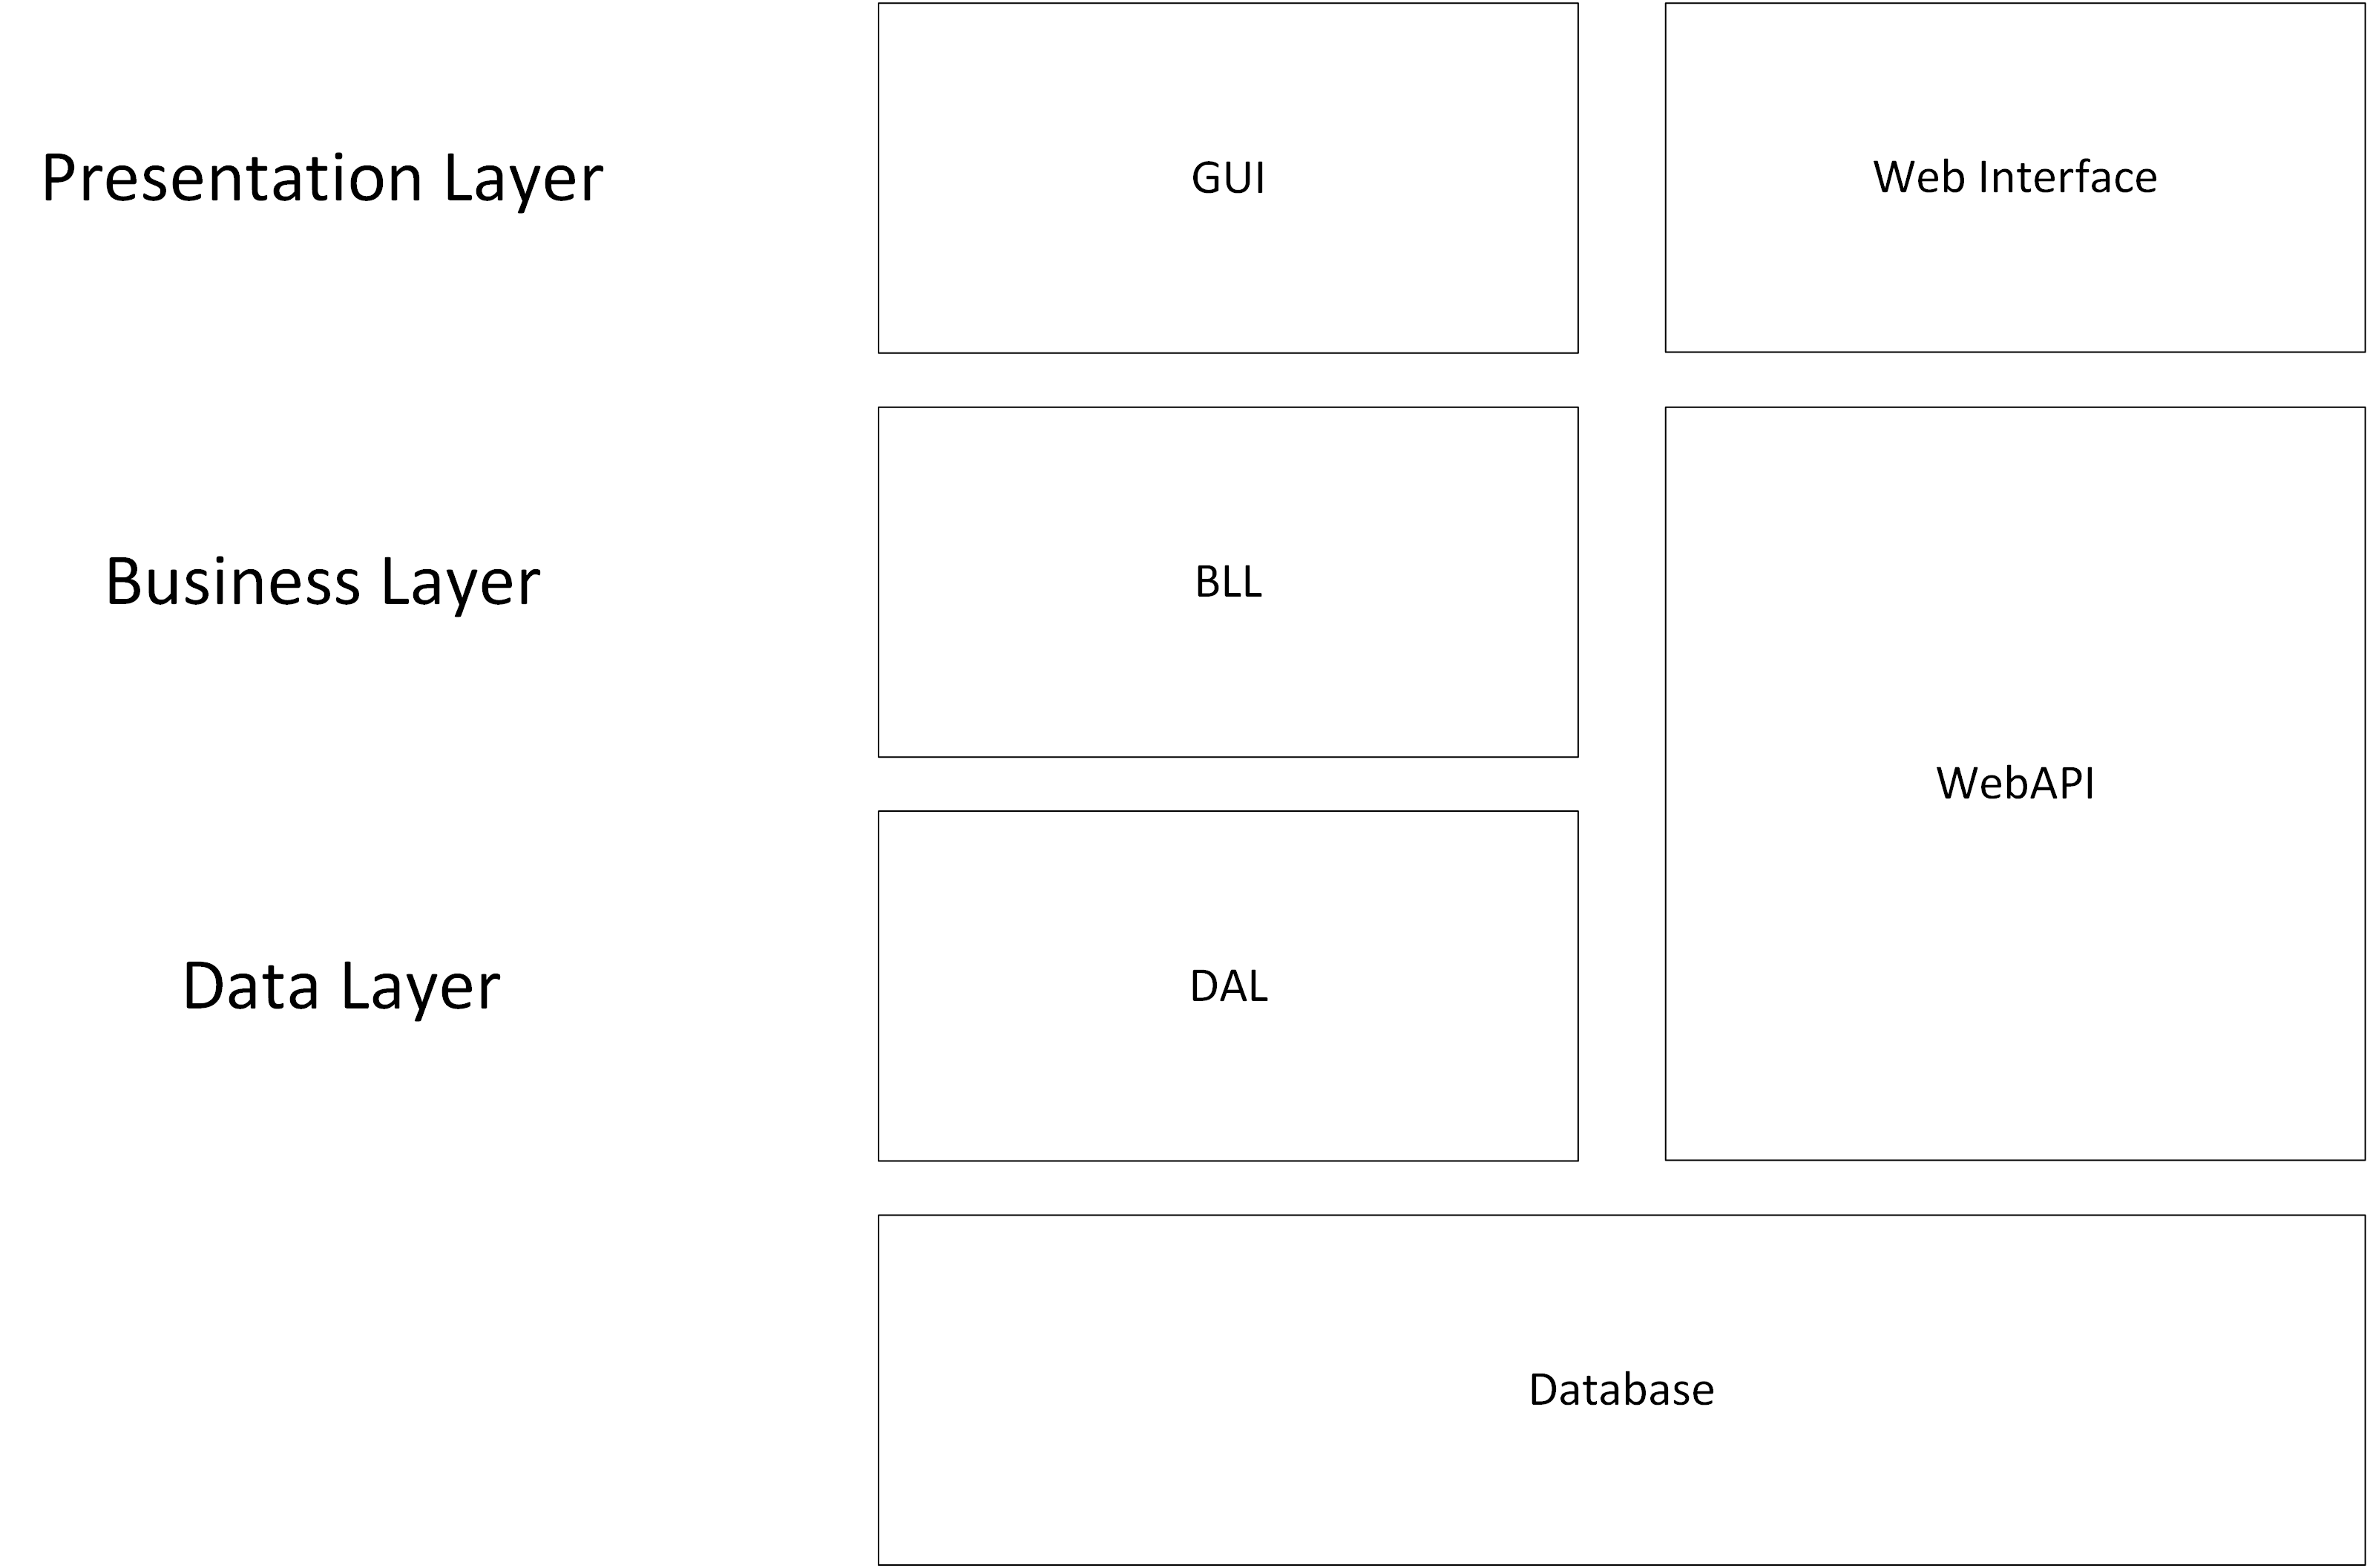
\includegraphics[width=0.75\textwidth]{Rapport/3tier}
	\caption{Overordnet system}
	\label{fig:ArkiDia}
\end{figure}

\subsection{N+1 view}
Arkitekturen er beskrevet med N+1, som er en specialisering af 4+1, der er beskrevet i artiklen af \cite{4plus1}. Specialiseringen gør det muligt at tilføje og fjerne de Views, som giver eller ikke giver mening for beskrivelsen af \gls{system}et. I systemarkitekturen er følgende Views indkluderet:
\begin{itemize}
	\item Domain View
	\item Use Case View
	\item Logical View
	\item Deployment View
	\item Data View
\end{itemize}
To af de listet Views: Domain View og Use Case View, er allerede beskrevet i afsnit~\ref{sec:specandanal}. Derfor vil følgende beskrivelser af disse kun være et sammendrag.

\subsubsection{Domain View}
Domain View bruger de fully-dressed \gls{usecase}s til at give et overblik over de ansvarsdomæner, som findes i systemet.

\subsubsection{Use Case View}
Use Case View er med til at skabe en overblik over, hvordan \gls{system}et skal interagere med brugeren.

\subsubsection{Logical View}
Logical View er en beskrivelse af, hvordan systemet er bygget op. Systemet består af to applikationer: et kasseapparatet og et web interface til administration. Begge applikationer er til dels lag-delt i tre lag: et Presentation Layer, et Business Layer og et Data Layer. Dette kan ses i figur~\ref{fig:ArkiDia}. De to applikationer er yderligere beskrevet i systemarkituren under afsnittet Logical View. 
\newline\newline
\textbf{Presentation Layer} er laget, som er tættest på brugeren. Det er her, hvor \gls{GUI} er placeret. \gls{GUI}. \gls{GUI} hjælpe brugeren igennem de funktionaliteter, som systemtet har, på den letteste måde.
%I dette lag bliver der introduceret begreber som \gls{View}, \gls{ViewModel} og \gls{Model} pga. \gls{MVVM}. \gls{MVVM} er et mønster, som adskiller funktionalitet og udseende. Dette gør at dele af brugergrænsefladen er testbar altså \gls{ViewModel}'s.
\newline\newline
\textbf{Business Layer} er laget, som indeholder \gls{BLL}. \gls{BLL} er hvor kasseapparatets funktionalitet kan findes. Det er dette lag, som f.eks. sørger for, at ordre og transaktioner bliver behandlet.
\newline\newline
\textbf{Data Layer} er laget, som indeholder \gls{DAL}. \gls{DAL} sørger for at skrive og læse fra databasen.
\newline\newline
\textbf{Web Interface og WebAPI} er en applikation for sig selv. Applikationen sørger for, at det er muligt at oprette, redigere og fjerne produkter fra kasseapparatet. Applikationen kan også vise statistik over salg i systemet. 

\subsubsection{Deployment View}
I Deployment View ses der, hvordan systemet kunne udrulles og sættes op. Her er det vigtig at bide mærke i, at selve databasen og \gls{WebAPI}'et kunne sættes op på deres egne separate computere fungerende som server, og GUI'en og business logikken, kunne køre på en anden computer, som så kunne kobles op til serveren. I vores system som det er udviklet, ligger databasen på samme computer som resten af systemet. \newline\newline
\begin{figure}[H]
	\centering
	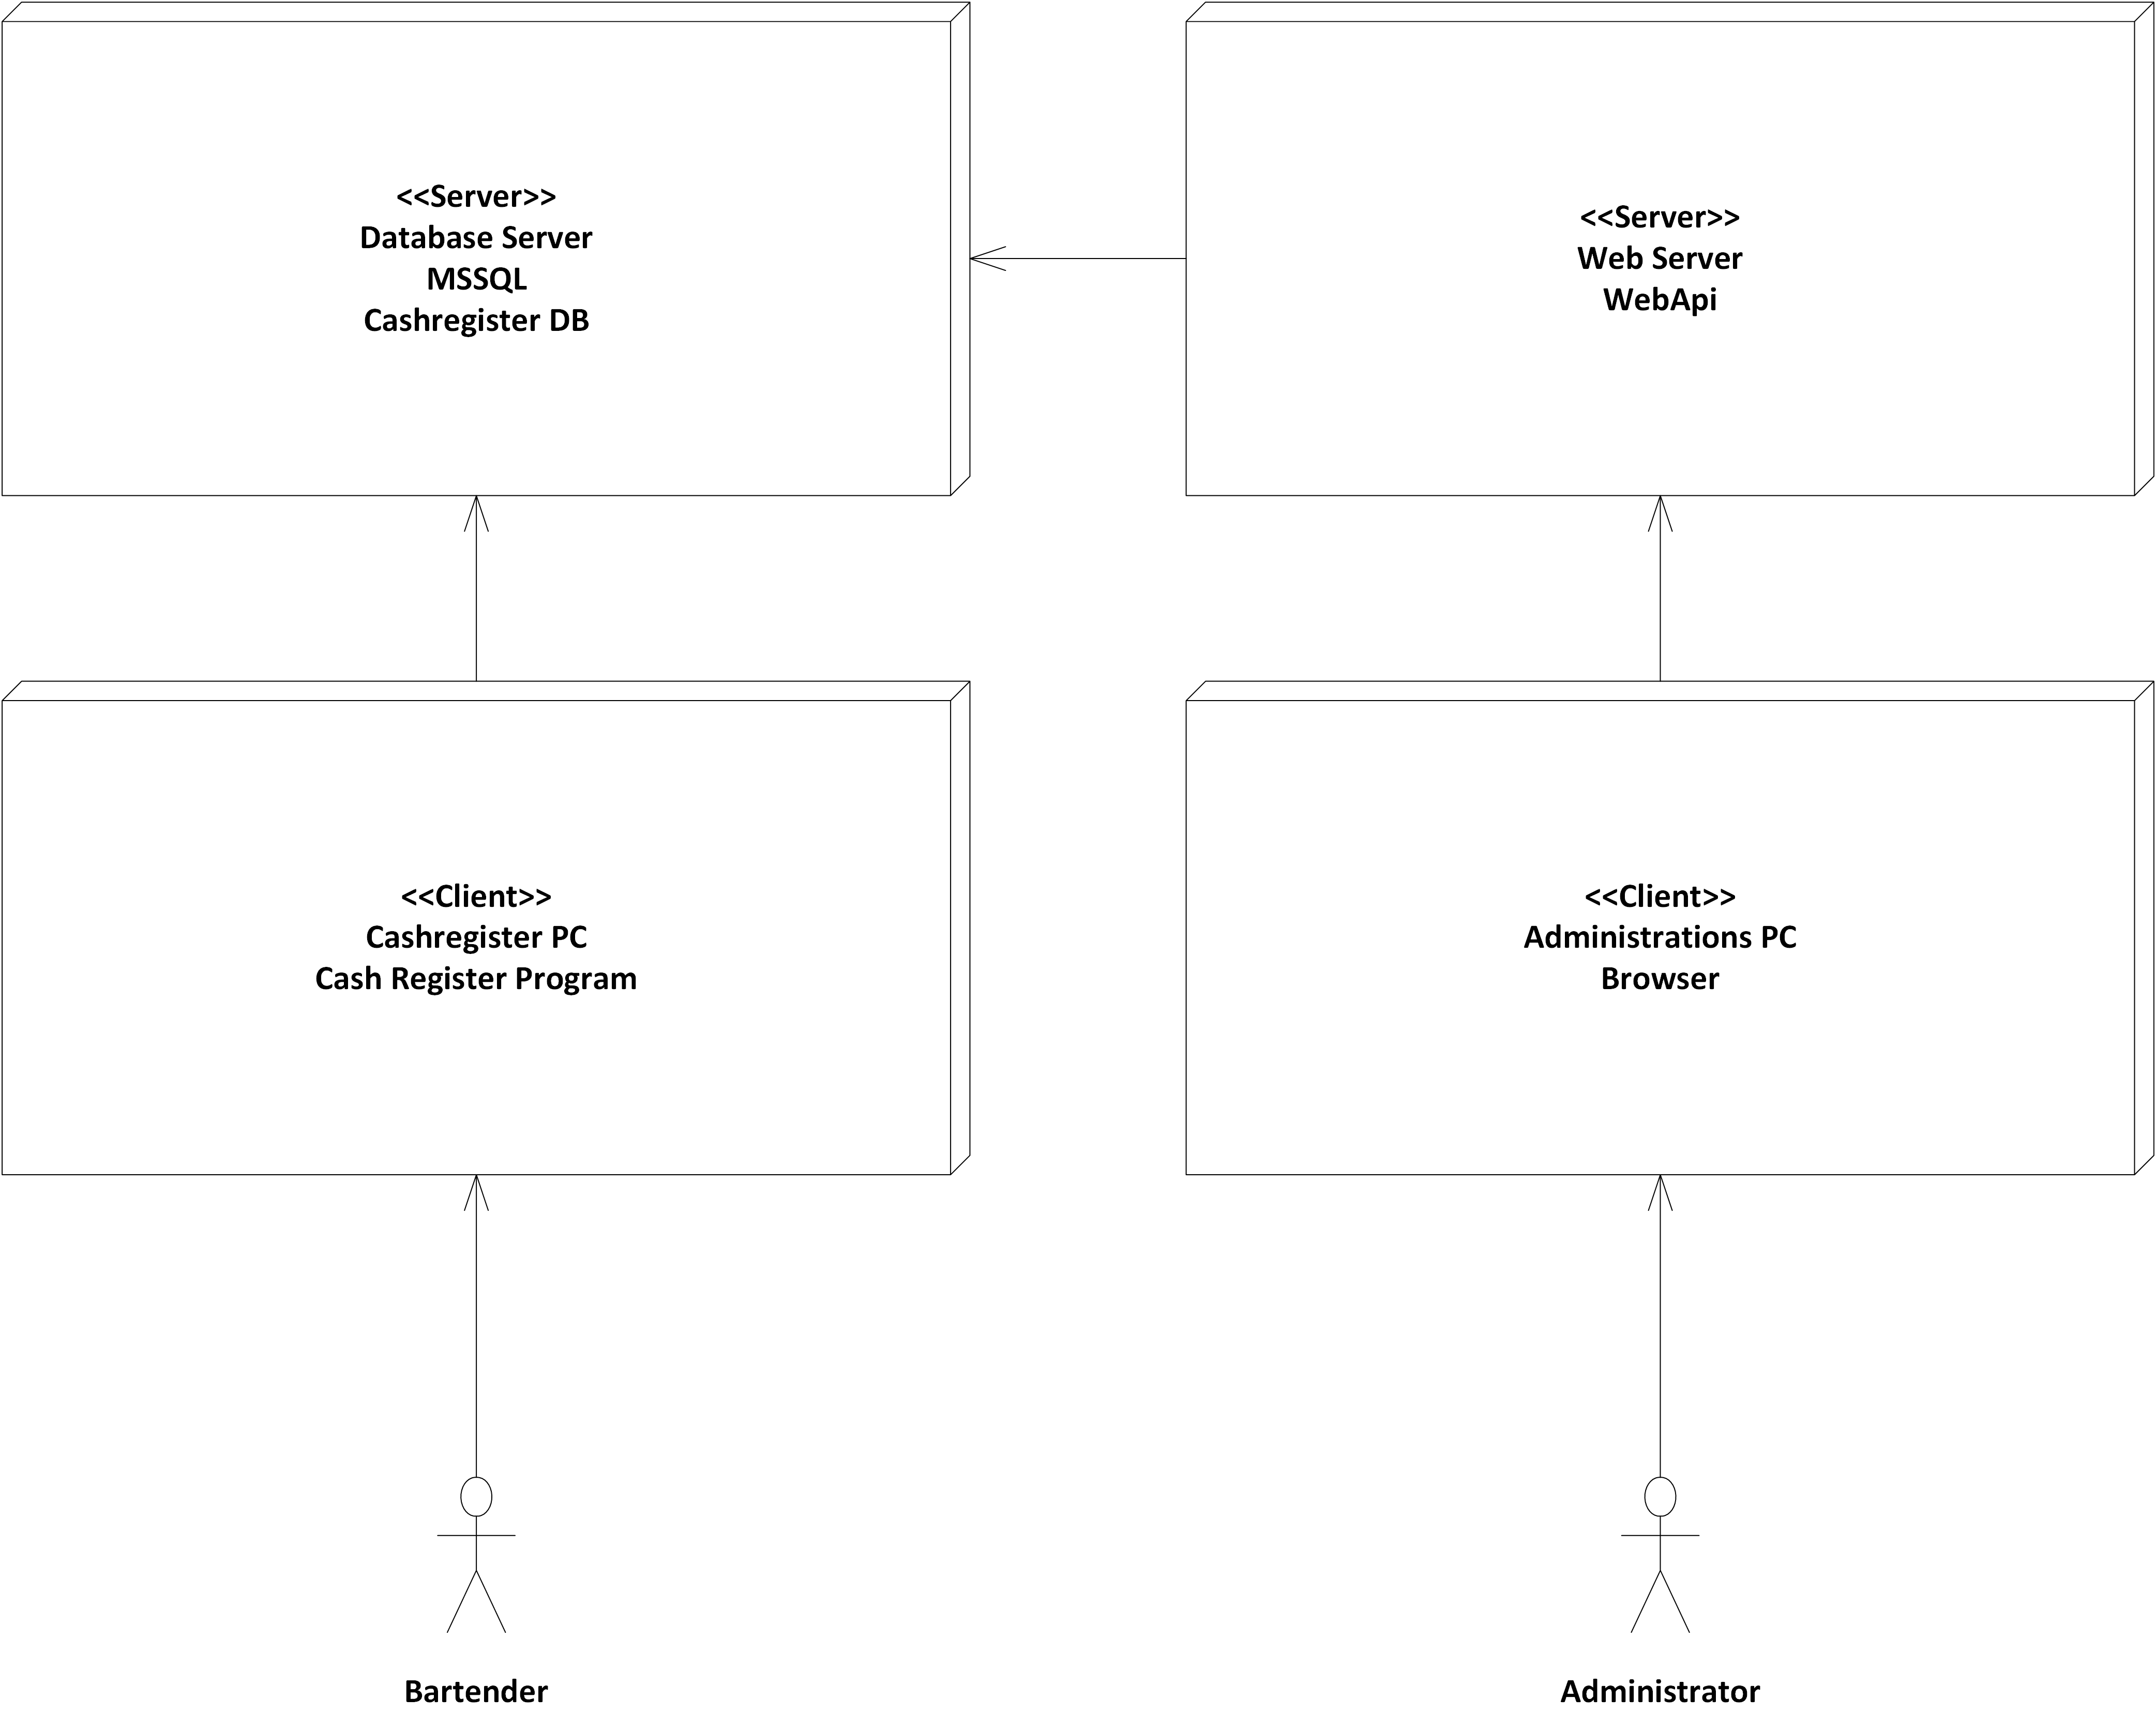
\includegraphics[scale=0.6]{/N+1/DeploymentView/System/Diagrammer/DEPLOY}
	\caption{Diagram over deployment af system}
	\label{fig:DeplayDia}
\end{figure}
Som det ses af figur \ref{fig:DeplayDia} kunne man sætte en administrations PC op, som ville koble op til en Web Server, som ville hoste Web API'et. Web API'et ville så tilkoble sig Database serveren, som ville køre på en separat server. Hertil ville CashRegister programmet så køre på en separat PC, som bartenderen ville have adgang til. Dette betyder, at man kunne opsætte flere kasseapparater, som kunne koble op til samme database.  

\subsubsection{Data View}
I Data View beskrives overgangen fra objekter i systemet til databasen. Her bliver en Mapping til databasen.\newline\newline
I dokumentationen er der beskrevet, hvor de forskellige klasser er blevet mappet til databasen. Her bliver der gennemgået, hvorfor tabellerne er sat op som de er, og hvordan deres forhold til hinanden er. Her er klassemodeller og de fysiske modeller sat op over for hinanden, så man hurtig kan se forskelle og ligheder.

\begin{figure}[H]
	\centering
	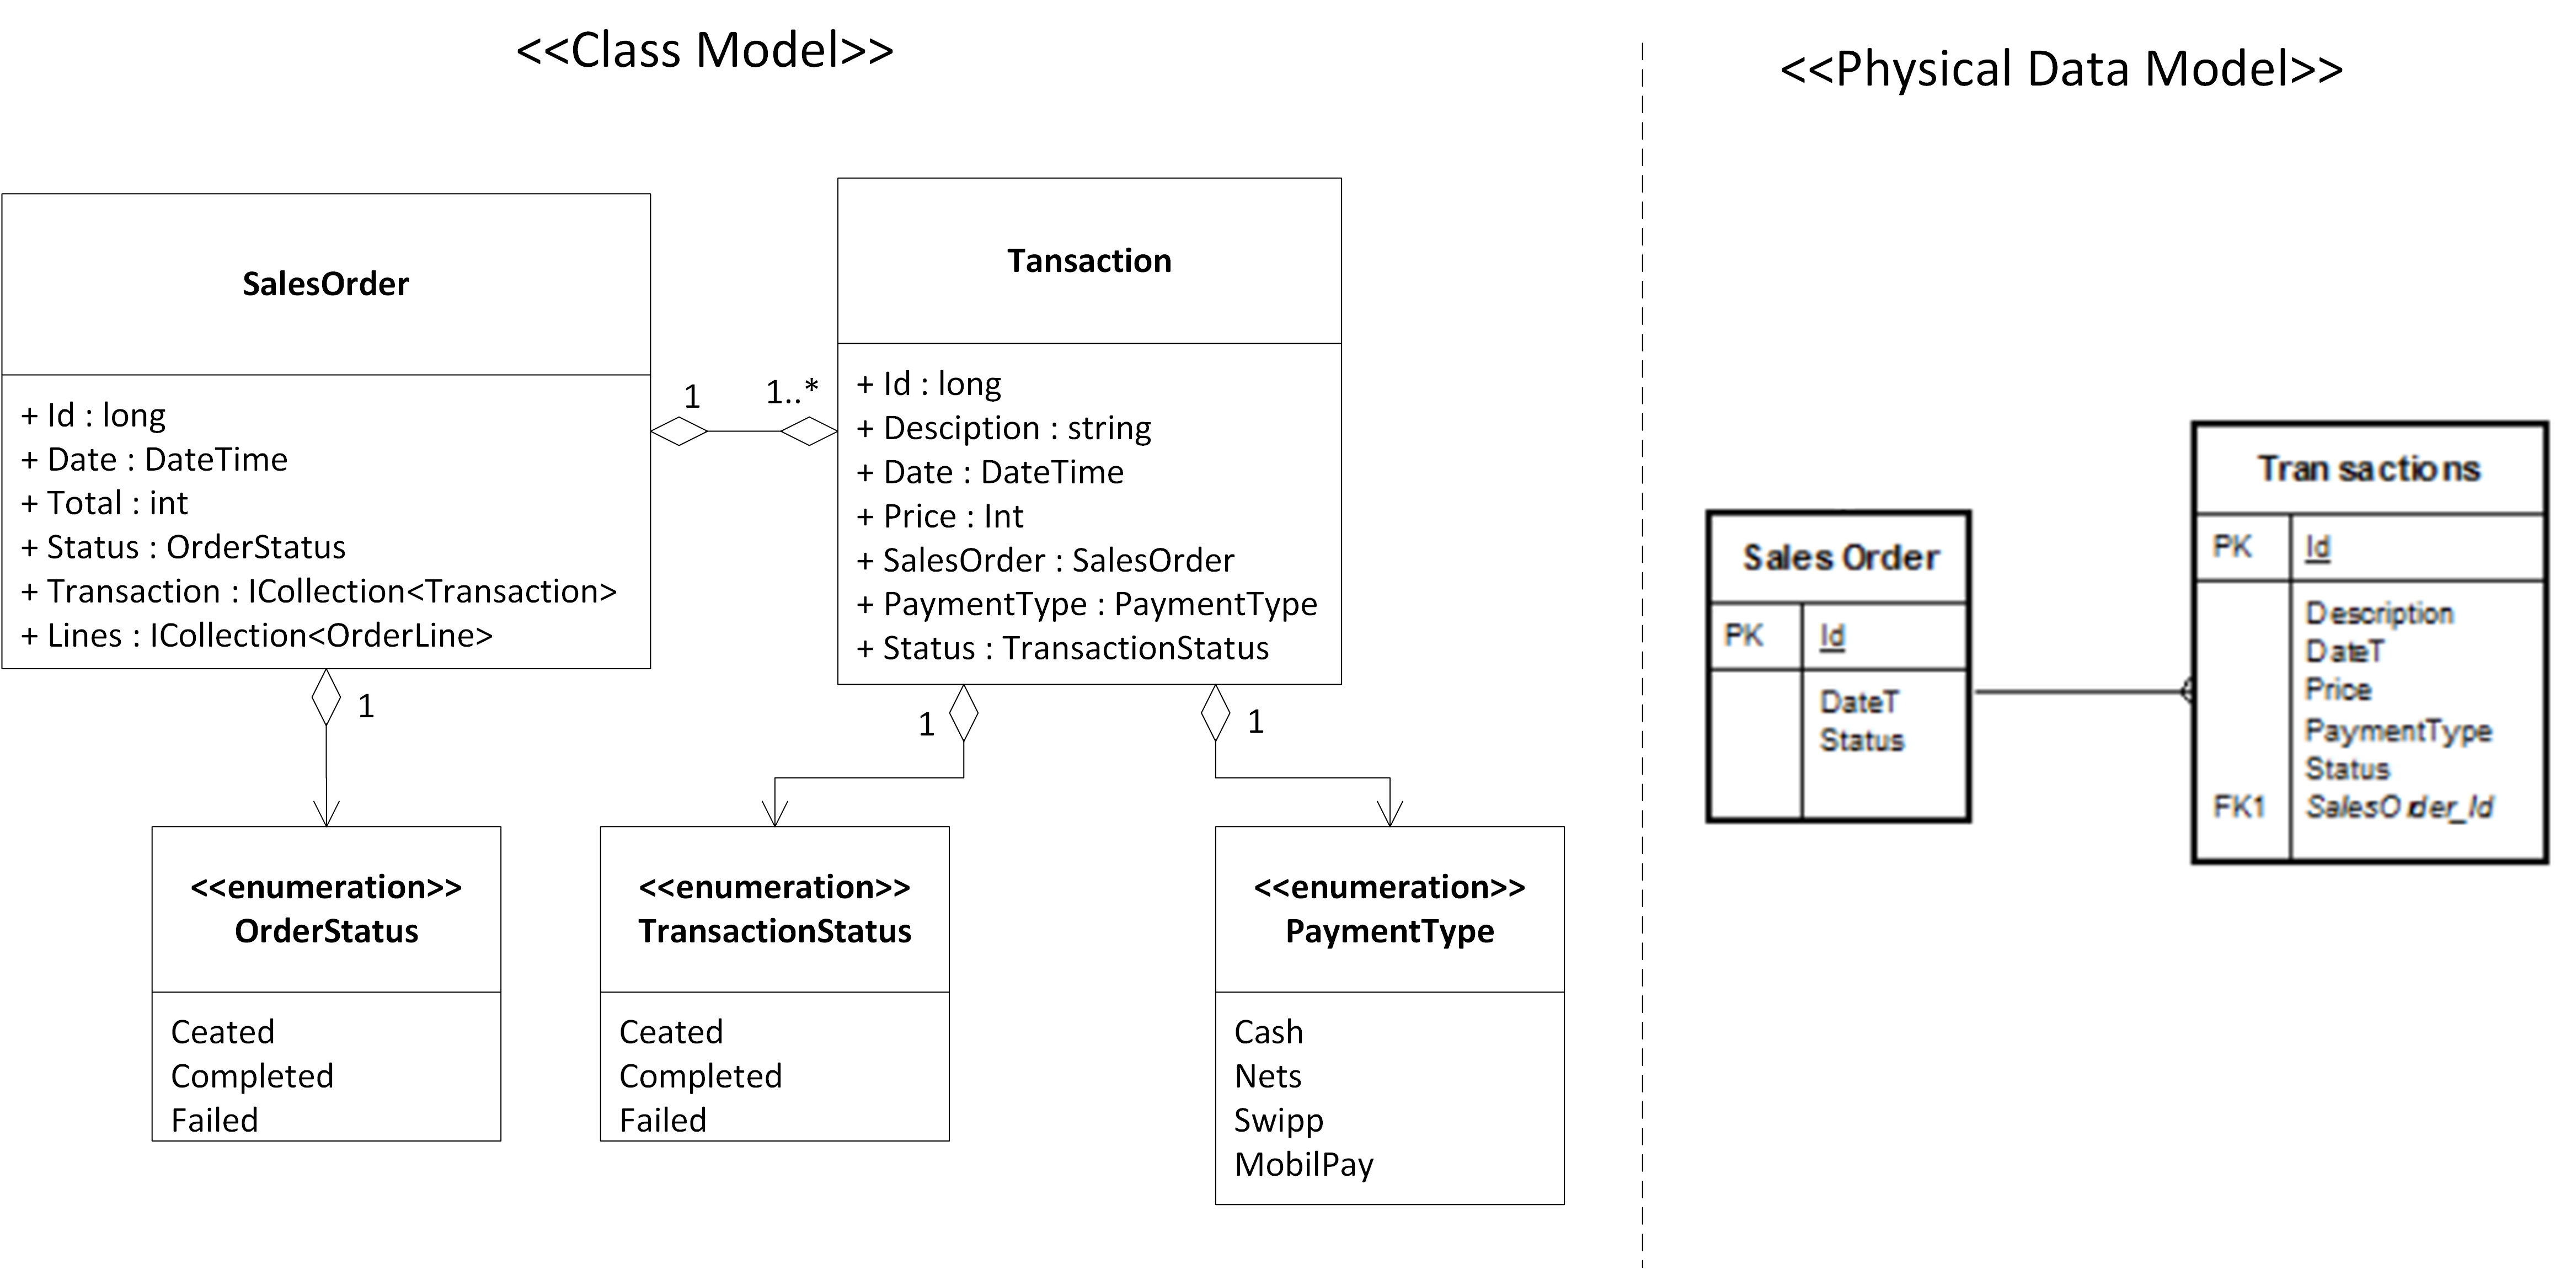
\includegraphics[scale=0.6]{/N+1/DataView/mapping/Mapping1}
	\caption{Diagram over objekt mapping}
	\label{MapDia}
\end{figure}	

På figur \ref{MapDia} ses det, hvordan kobling af SalesOrder sker til Databasen. Her kan det ses, at der mellem SalesOrder og Transaction er et one-to-many forhold, og at Transaction har en fremmed nøgle til SalesOrder.\newline\newline
Ydermere kan der i Data View ses, hvordan dataflows sker fra én handling til den næste. Hertil er der lavet nogle aktivitetsdiagrammer ud fra de definerede Use Cases. 

\begin{figure}[H]
	\centering
	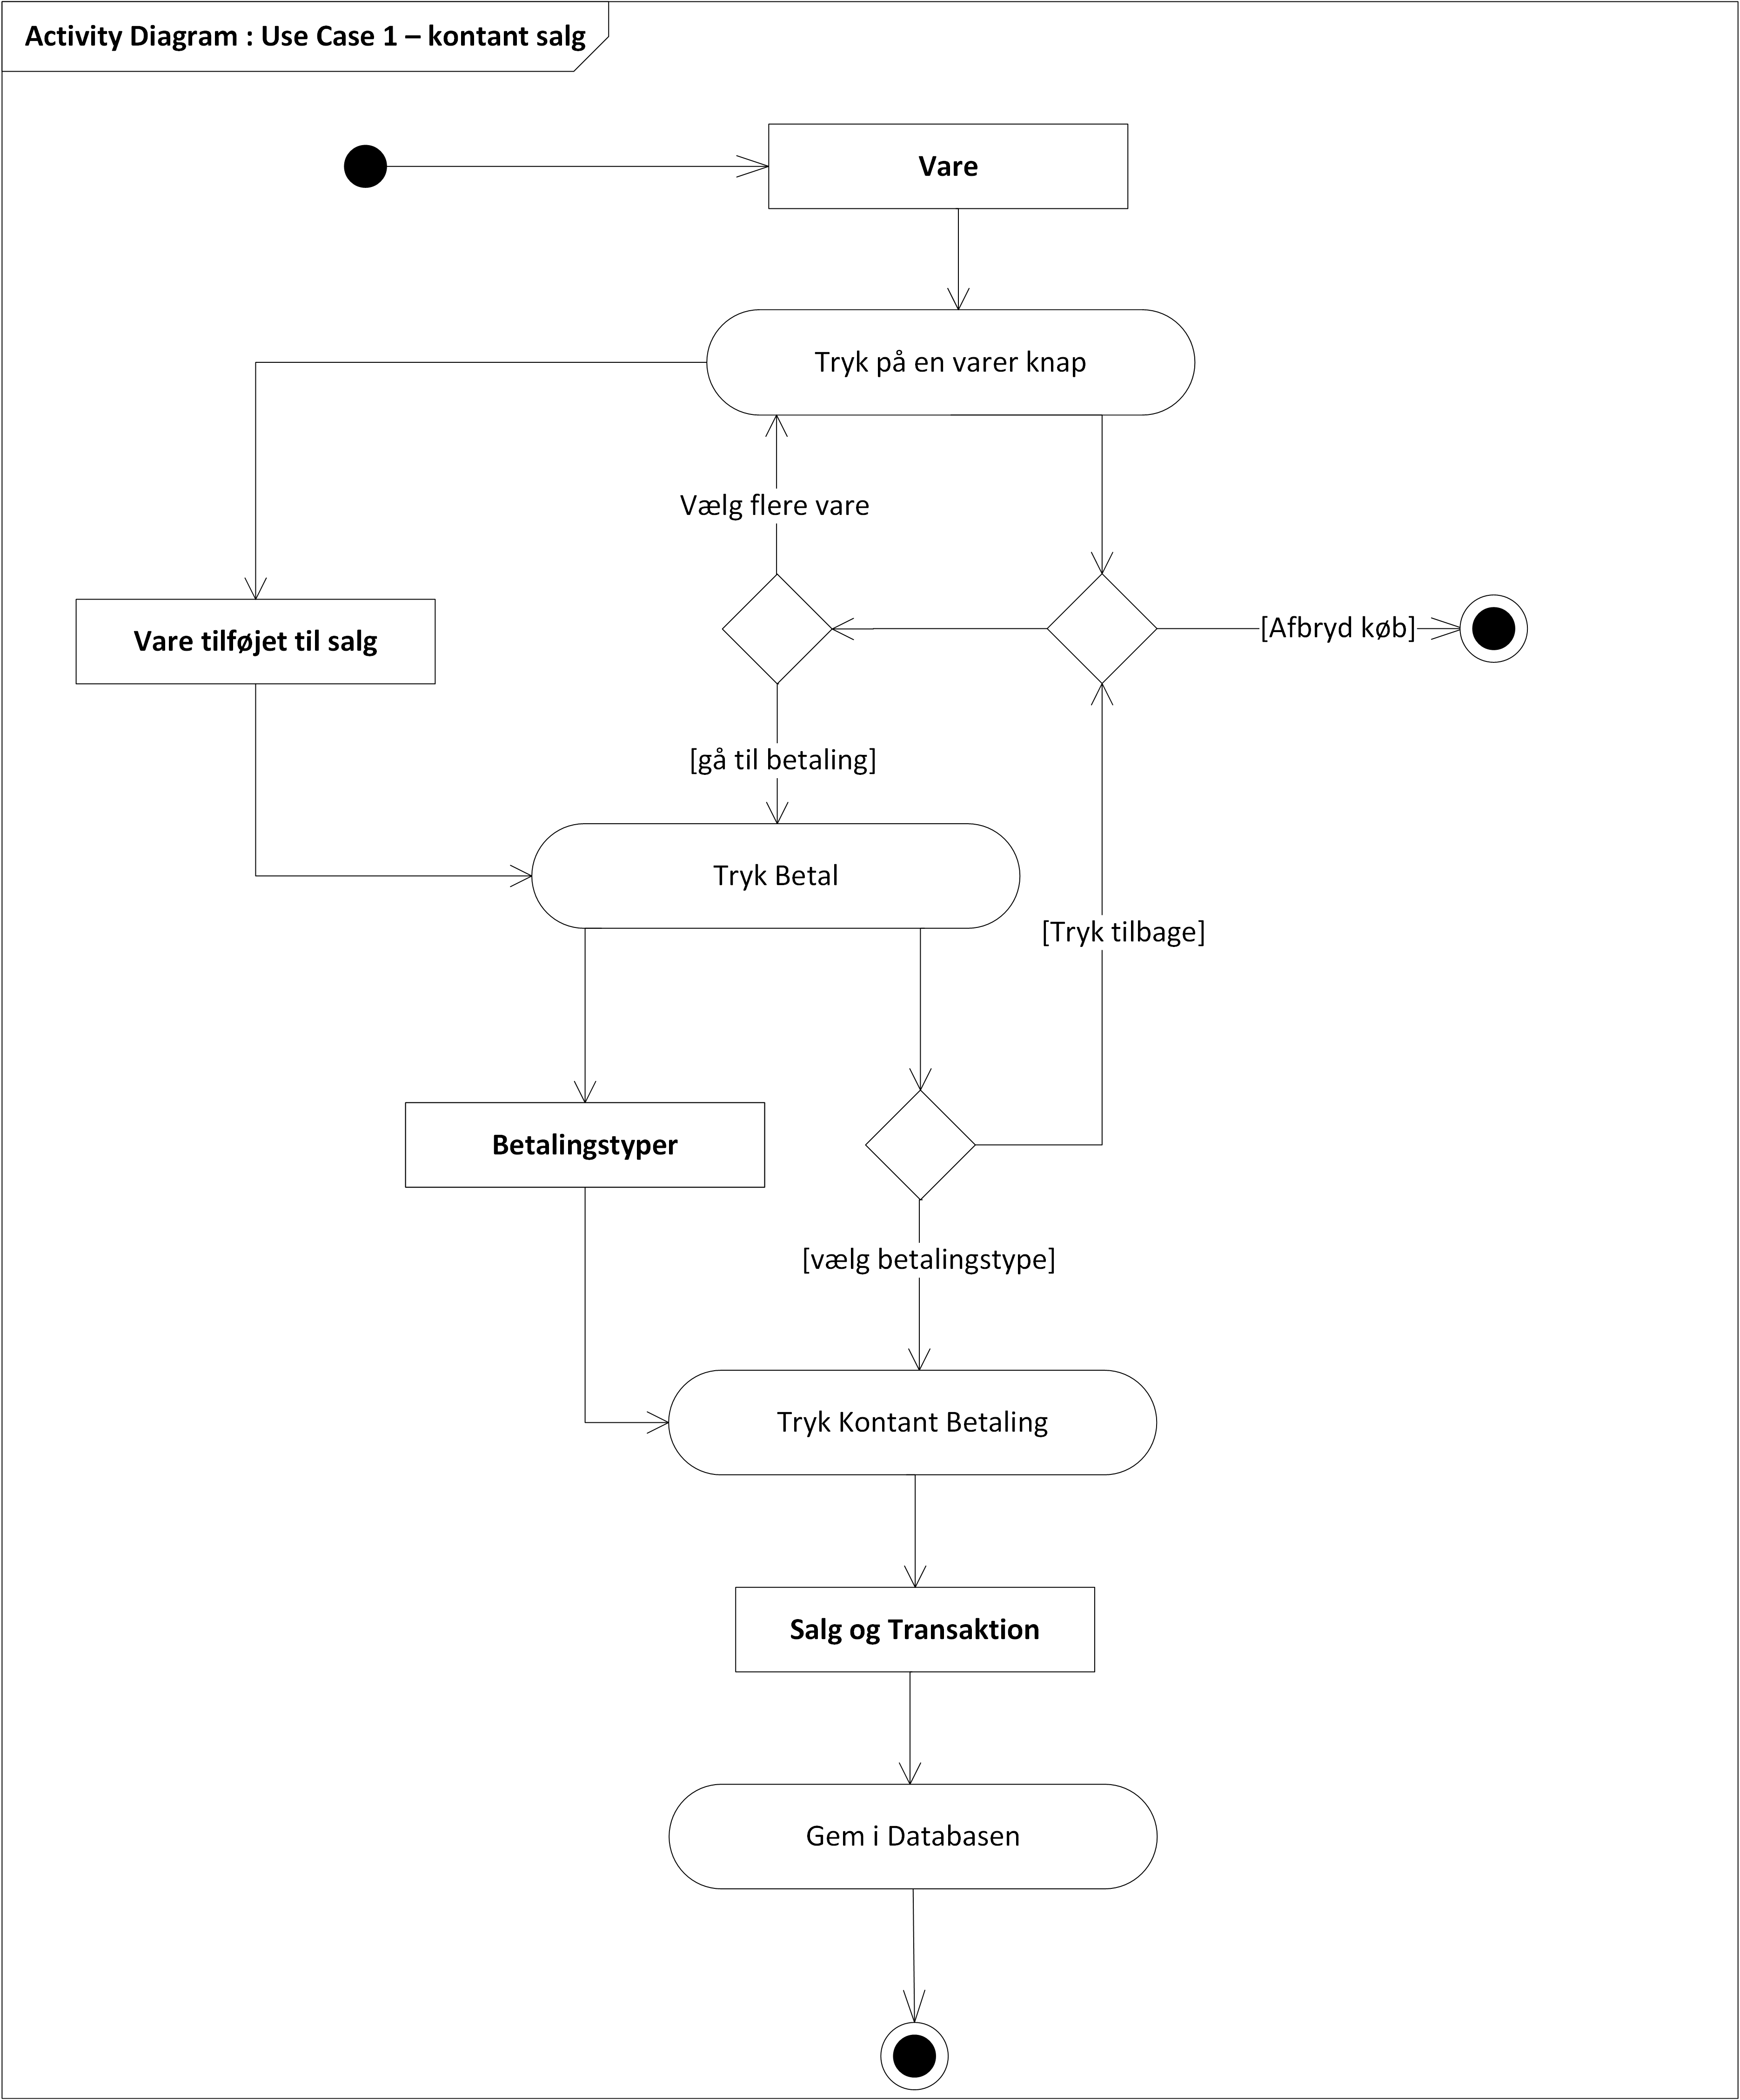
\includegraphics[scale=0.6]{/N+1/DataView/DataFlow/UC1}
	\caption{Aktivitetsdiagram over Use Case 1}	
	\label{AktDia}
\end{figure}

På figur \ref{AktDia} er dataflowet i forhold til Use Case 1 illustreret via et aktivitetsdiagram. Aktiviteterne gentages i nogle tilfælde og kører derfor i en løkke, og det kan også ses hvornår Use Casen og, hvordan Use Casen afsluttes. Alt dette står mere detaljeret beskrevet i dokumentationen. 